
\subsection{Alligatoridae --- Alligators}
\begin{center}
\begin{longtabu} to \textwidth {| | p{3.5cm} | X | |}

	\hline
	Taxonomy/Ancestry &
	subfamilies:
	\begin{itemize}[noitemsep]
		\item \textbf{alligatorinae} -- true alligators; only 1 of 10 genera currently extant; represented today by \emph{A. mississippiensis} in US and \emph{A. Sinesis} in China
		\item \textbf{caimaninae} -- caimans in C. and S. America
	\end{itemize}
	
	\begin{center} 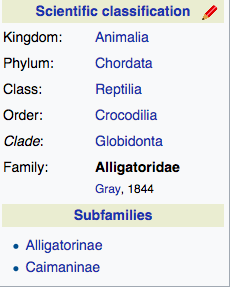
\includegraphics[scale=0.5]{crocodylia/alligatoridae/taxonomy} \end{center}
	 \\
	\hline
	Size & 
	alligator: 5-20 ft (1.5-6.1 m)
	
	caiman: average maximum weight of 6 to 40 kg (13 to 88 lb) depending on species, with the exception of the black caiman (Melanosuchus niger), which can grow more than 5 m (16 ft) in length and weigh up to 1,100 kg (2,400 lb). The average length for most of the other caiman species is about 2 to 2.5 m (6.6 to 8.2 ft) long. largest species = black caiman, smallest = Cuvier's dwarf.
	\\
	\hline
	Color &
	
	 \\
	\hline
	Anatomy &
	\begin{itemize}[noitemsep]
		\item diapsid skull
		\item armored w/ osteoderms and large scales that do not overlap
		\item forelimbs are smaller and weaker with 5 partially-webbed toes
		\item distinguishing from crocodiles:
			\begin{itemize}[noitemsep]
				\item wider, shorter heads w/ more obtuse snouts
				\item 4th enlarged underjaw tooth fits into pit in upper jaw --> no teeth visible when mouth closed
				\item no jagged fringe on hind legs + feet
				\item sensory pits appear only on snout and face, not neck and body
				\item toes of hind feet webbed not more than halfway to tips
				\item intolerant to salinity
				\item generally less aggressive and dangerous
				\item partake in foliage and fruit in addition to fish and meat
			\end{itemize}
		\item caiman characteristics:
			\begin{itemize}[noitemsep]
				\item no bony septum b/w nostrils
				\item ventral armour composed of overlapping bony scutes formed from two parts united by a suture
				\item longer, more slender, teeth than those possessed by alligators. The calcium rivets on its scales make their hides stiffer, and thus less valuable, than those of alligators and crocodiles.
			\end{itemize}
	\end{itemize}
				
	 \\
	\hline
	Dimorphism & 
	males larger and grow faster.
	
	\\
	\hline
	Behavior & 
	\begin{itemize}[noitemsep]
		\item ectotherms basking on shoreline
		\item float on surface of water
		\item become more subdued as temperatures drop but do not hibernate, making use of burrows in the winter months
		\item live in groups w/ dominance hierarchies. the highest-ranking individuals assert dominance through ritualized behaviors such as vocalizations and slapping the water with their heads.
		\item \textbf{high walk}: 4-limbed forward motion used for overland travel w/ belly up from the ground
		\item alligator holes in the wetlands increase plant diversity and provide habitats for other animals during droughts
		
	\end{itemize}
	\\
	\hline
	Habitat & 
	lakes, slow-moving streams/rivers, rivers, swamps, marshes, occasionally roadside ditches. freshwater sites w/ slow or still waters. often inhabit heavily-vegetated areas w/ muddy or murky water.
	\\
	\hline
	Distribution & 
	a New World group w/ habitats in Central-Northern S. America; parts of southern and western Central America and Mexico; SE United States; eastern China.
	\\
	\hline
	Feeding Ecology & 
	\begin{itemize}[noitemsep]
		\item opportunistic scavenger-hunters
		\item juveniles mainly eat snails and other invertebrates
		\item Typical adult diet = fish, small mammals, other reptiles (including smaller alligatorids), and birds, occasionally continuing to eat snails/invertebrates
		\item Predation typically occurs among eggs and hatchlings
		\item Racoons, coati, foxes, skunks, and other mammals, snakes, and various raptors, can raid nests or take hatchlings
		\item occasional cannibalism, but rare
		\item larger alligators help control coypu population
	\end{itemize}
	\\
	\hline
	Reproductive Biology & 
	\begin{itemize}[noitemsep]
		\item spring reproductive season
		\item courtship rituals thru loud bellowing choruses, vibrations of the male trunk
		\item use vegetables to construct nest mounds
		\item 12-60 eggs depending on species
		\item egg-laying once a year in midsummer, w/ eclosion 1-2 months afterward
		\item females respond to noises from eggs and assist offspring. offspring also use egg teeth for eclosion.
		\item females remain w/ offspring for up to 1 year.
		\item TSD is associated w/ several species, such as American alligator and common caimans. <88degF/31degC = female; >90degF/32degC = male. natural sex ratio of 5:1 female:male.
		\item Muja = oldest known in Serbia
	\end{itemize}
	\\
	\hline
	Conservation Status & 
	\begin{itemize}[noitemsep]
		\item raised commercially for their meat and skin
		\item ecotourism industry
		\item in Louisiana, heavy grazing by coypu and muskrat are damaging coastal wetlands
		\item Chinese alligator critically endangered; Louisiana and Florida zoos have some in captivity they are trying to preserve
	\end{itemize}
	\\
	\hline
\end{longtabu}
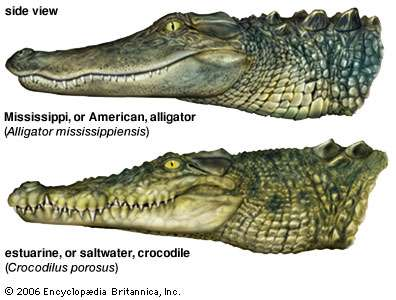
\includegraphics[scale=0.5]{crocodylia/alligatoridae/side.jpg}
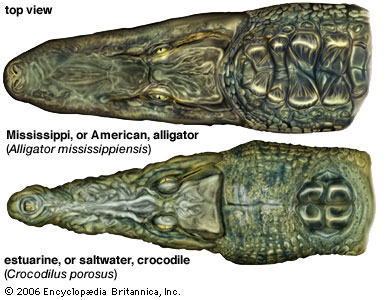
\includegraphics[scale=0.5]{crocodylia/alligatoridae/top.jpg}

\end{center}
